% Abbildung: Die fuenf Kompositionsoperatoren der Faust-Blockdiagrammalgebra.
% Ergaenzung zu Tabelle 3.1 in Abschnitt 3.3.
%
% Uebersetzen:  pdflatex abb-faust-operatoren.tex -> abb-faust-operatoren.pdf
% Einbinden:    \includegraphics[width=\textwidth]{abb-faust-operatoren}
%
% Aufbau: fuenf Zeilen mit festem Abstand (\rowpitch). Alle Bloecke, Pfeile
% und Beschriftungen stehen in denselben Spalten (\colin, \colone, \coltwo,
% \colout, \coltext), damit die Zeilen untereinander fluchten.
\documentclass[border=4pt]{standalone}
\usepackage[utf8]{inputenc}
\usepackage[T1]{fontenc}
\usepackage{tikz}
\usetikzlibrary{arrows.meta}

% ---- Raster ----------------------------------------------------------
\def\rowpitch{1.8}   % vertikaler Abstand der Zeilen in cm
\def\colin{0.30}     % Beginn des Eingangspfeils
\def\colone{1.35}    % erste Blockspalte
\def\coltwo{3.15}    % zweite Blockspalte
\def\colout{4.65}    % Ende des Ausgangspfeils
\def\coltext{5.05}   % Beginn der Beschriftungsspalte

\begin{document}
	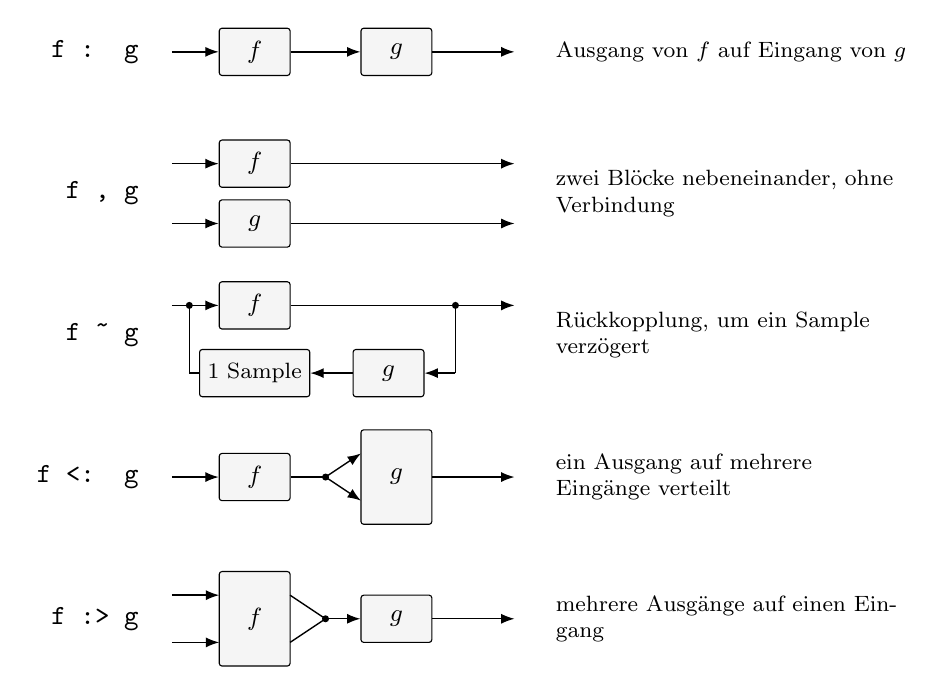
\begin{tikzpicture}[
		font=\small,
		blk/.style={draw,rounded corners=1pt,minimum width=9mm,minimum height=6mm,
			inner sep=2pt,fill=black!4},
		w/.style={-{Latex[length=1.7mm]},line width=0.5pt},
		p/.style={line width=0.5pt},
		dot/.style={circle,fill=black,inner sep=0.9pt},
		lbl/.style={font=\ttfamily,anchor=east},
		txt/.style={font=\footnotesize,anchor=west,align=left,text width=45mm}]
		
		% ============ 1) Sequenziell:  f : g ============
		\begin{scope}[yshift=0cm]
			\node[lbl] at (0,0) {f : g};
			\node[blk] (f) at (\colone,0) {$f$};
			\node[blk] (g) at (\coltwo,0) {$g$};
			\draw[w] (\colin,0) -- (f);
			\draw[w] (f) -- (g);
			\draw[w] (g) -- (\colout,0);
			\node[txt] at (\coltext,0) {Ausgang von $f$ auf Eingang von $g$};
		\end{scope}
		
		% ============ 2) Parallel:  f , g ============
		\begin{scope}[yshift=-\rowpitch cm]
			\node[lbl] at (0,0) {f , g};
			\node[blk] (f2) at (\colone,0.38) {$f$};
			\node[blk] (g2) at (\colone,-0.38) {$g$};
			\draw[w] (\colin,0.38) -- (f2);   \draw[w] (f2) -- (\colout,0.38);
			\draw[w] (\colin,-0.38) -- (g2);  \draw[w] (g2) -- (\colout,-0.38);
			\node[txt] at (\coltext,0) {zwei Blöcke nebeneinander, ohne Verbindung};
		\end{scope}
		
		% ============ 3) Rekursiv:  f ~ g ============
		% Signalweg der Rueckkopplung: Abgriff hinter f, nach unten, nach links
		% durch g und die Verzoegerung, wieder hinauf auf den Eingang von f.
		\begin{scope}[yshift=-2*\rowpitch cm]
			\node[lbl] at (0,0) {f \textasciitilde{} g};
			\node[blk] (f3) at (\colone,0.38) {$f$};
			\node[blk] (g3) at (3.05,-0.48) {$g$};
			\node[blk,minimum width=14mm] (d3) at (\colone,-0.48) {\footnotesize 1 Sample};
			\draw[w] (\colin,0.38) -- (f3);
			\draw[p] (f3) -- (3.9,0.38);
			\draw[w] (3.9,0.38) -- (\colout,0.38);
			% Abgriff und Rueckweg
			\draw[p] (3.9,0.38) -- (3.9,-0.48);
			\draw[w] (3.9,-0.48) -- (g3);
			\draw[w] (g3) -- (d3);
			\draw[p] (d3) -- (0.52,-0.48) -- (0.52,0.38);
			\node[dot] at (0.52,0.38) {};
			\node[dot] at (3.9,0.38) {};
			\node[txt] at (\coltext,0) {Rückkopplung, um ein Sample verzögert};
		\end{scope}
		
		% ============ 4) Split:  f <: g ============
		\begin{scope}[yshift=-3*\rowpitch cm]
			\node[lbl] at (0,0) {f <: g};
			\node[blk] (f4) at (\colone,0) {$f$};
			\node[blk,minimum height=12mm] (g4) at (\coltwo,0) {$g$};
			\draw[w] (\colin,0) -- (f4);
			\draw[p] (f4) -- (2.25,0);
			\node[dot] at (2.25,0) {};
			\draw[w] (2.25,0) -- (2.7,0.3);
			\draw[w] (2.25,0) -- (2.7,-0.3);
			\draw[w] (g4) -- (\colout,0);
			\node[txt] at (\coltext,0) {ein Ausgang auf mehrere Eingänge verteilt};
		\end{scope}
		
		% ============ 5) Merge:  f :> g ============
		\begin{scope}[yshift=-4*\rowpitch cm]
			\node[lbl] at (0,0) {f :> g};
			\node[blk,minimum height=12mm] (f5) at (\colone,0) {$f$};
			\node[blk] (g5) at (\coltwo,0) {$g$};
			\draw[w] (\colin,0.3) -- (0.9,0.3);
			\draw[w] (\colin,-0.3) -- (0.9,-0.3);
			\draw[p] (1.8,0.3) -- (2.25,0);
			\draw[p] (1.8,-0.3) -- (2.25,0);
			\node[dot] at (2.25,0) {};
			\draw[w] (2.25,0) -- (g5);
			\draw[w] (g5) -- (\colout,0);
			\node[txt] at (\coltext,0) {mehrere Ausgänge auf einen Eingang};
		\end{scope}
		
	\end{tikzpicture}
\end{document}